\chapter{Basics}
\section{Opening and creating new image}
Let's start with opening an image, you have to go to 'File' and you're either going to 'Open' then choose an image and click 'OK'.\\
\\
But when you going to 'File' and choose 'New', you'll be presented this with screen..\\
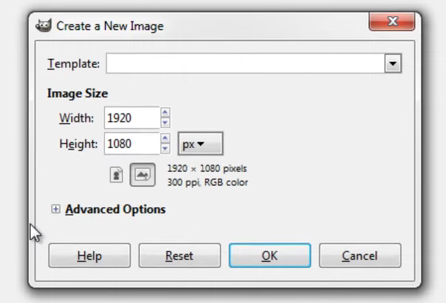
\includegraphics{new} \\
.. asking you what the width and hight of the image you'll going to be creating will be.\\
you can choose a template, these will give little templates for most monitors like these..\\
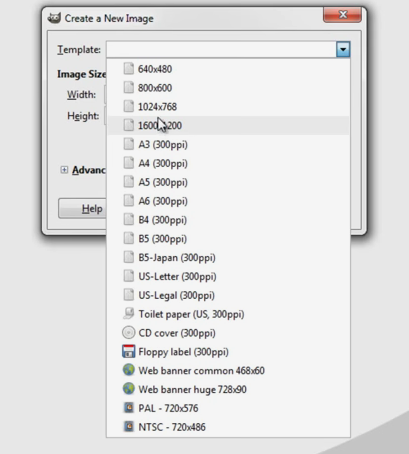
\includegraphics{template} \\
you can choose between pixels, inches, millimeters, points and anything else it there.
you can choose if you want to it landscape or portrait so fortunate would be the hight is bigger than the width, and a landscape is the width is bigger than the hight.\\
Finally, click 'OK' and you are presented with the blank canvas. So now you can do whatever you want.

\section{Image Cropping, Resizing, and Saving in JPEG Format }
\subsection{Cropping}
\subsection{Resizing}
\subsection{Saving}